\chapter{Related Work}

The area of relational learning on semantic web has recently attracted interest from many researchers. The approaches that aim at tackling this problem can be mainly classified into two groups: statistics-based and logic-based. In this chapter we review semantic web and the relevant works from these groups.

\section{Semantic Web}

The Semantic Web enables computers to interpret the meaning of the data all over the Internet. Alternatively, it can be defined as "a web of data that can be processed directly and indirectly by machines" in~\cite{ref26}.

The World Wide Web Consortium (W3C) defines semantic web and the Resource Description Framework (RDF) as a platform for Linked Data~\cite{ref26}. The W3C proposes other technologies such as SPARQL, OWL for data manipulation. Architecture of the W3C can be presented as a stack in Figure~\ref{fig1}~\footnote{\url{https://www.w3.org/DesignIssues/diagrams/sweb-stack/2006a.png}}.

\begin{figure}
\centering
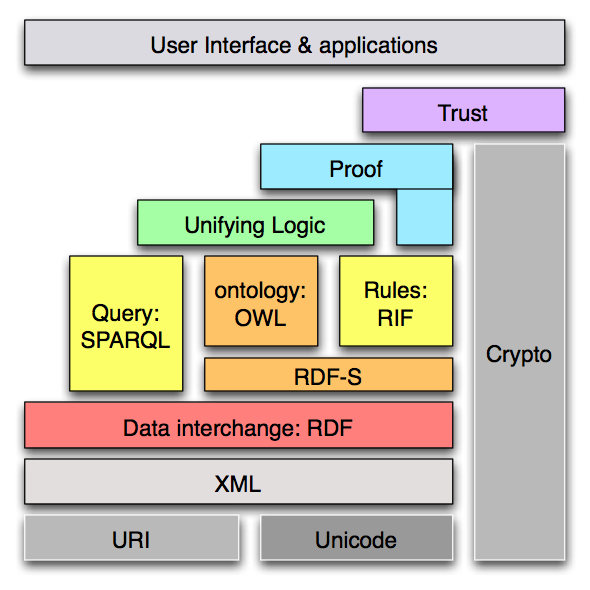
\includegraphics[width=0.65\textwidth]{semantic-web.png}
\caption{The Semantic Web technologies}
\label{fig1}
\end{figure}

The RDF can be used to describe knowledge graph where facts are presented in a format: \textit{$<$subject$>$ $<$predicate$>$ $<$object$>$}. This is the fundamental format of many knowledge bases such as YAGO~\cite{ref28}, FreeBase~\footnote{\url{https://developers.google.com/freebase/}}, Wikidata\footnote{\url{https://www.wikidata.org}}, etc. There are several typical knowledge graphs listed in Table~\ref{table1}~\cite{ref27} which have various scales. Of all the KB mentioned in the table, Google's Knowledge Graph is the largest with 18 billions facts. In our current work, we pay attention to YAGO, IMDB for experimental results.

Though having different number of predicates, entities and facts, these graphs share the following common properties~\cite{ref27}:

\begin{itemize}
\item Facts from real world are reflected in the knowledge graphs.
\item The domains are fruitful in the knowledge graphs, e.g, sports, arts, ...
\item The interconnection between knowledge graphs are taken into consideration, i.e, the mapping of entities and relations are explicitly indicated in each KB.
\end{itemize}

\begin{table}
\begin{center}
\begin{tabular}{|c|c|c|c|c|}
\hline
Name & Instances & Facts & Types & Relations\\
\hline\hline
DBpedia (English) & 4,806,150 & 176,043,129 & 735 & 2,813\\
\hline
YAGO & 4,595,906 & 25,946,870 & 488,469 & 77\\
\hline
Freebase & 49,947,845 & 3,041,722,635 & 26,507 & 37,781\\
\hline
Wikidata & 15,602,060 & 65,993,797 & 23,157 & 1,673\\
\hline
NELL & 2,006,896 & 432,845 & 285 & 425\\
\hline
OpenCyc & 118,499 & 2,413,894 & 45,153 & 18,526\\
\hline
Google's Knowledge Graph & 570,000,000 & 18,000,000,000 & 1,500 & 35,000\\
\hline
Google's Knowledge Vault & 45,000,000 & 271,000,000 & 1,100 & 4,469\\
\hline
Yahoo! Knowledge Graph & 3,443,743 & 1,391,054,990 & 250 & 800\\
\hline
IMDB & & & & \\
\hline
\end{tabular}
\end{center}
\caption{List of typical knowledge graphs}
\label{table1}
\end{table}

\section{Statistics-based Approaches}

The statistics-based approaches focus on building models with latent features which are not directly observable from the original data~\cite{ref1}. The core idea is to infer correlation between objects based on selected hidden features. Besides, feature extraction is automatically executed in these methods.

RESCAL is one of principal algorithms in this direction where relations of all hidden feature pairs are taken into consideration~\cite{ref2, ref3}. This method is extended to classical tensor decomposition algorithm~\cite{ref4} and neural tensor network~\cite{ref5}.

While many tensor factorization methods use subject, predicate and object as three dimensions to model a knowledge graph as a cube, some matrix decomposition algorithms try to transform this cube into two dimensional data. For instance, in~\cite{ref6, ref7} subject and object dimensions are merged into one representing a pair of entities.

Distance-based models use the intuition that entities have high chance to be related to each other if their hidden representation features are close to each other. The closeness can be checked based on some predefined distance measures. This approach can be expanded to structure embedding model~\cite{ref8}.

\section{Logic-based Approaches}

The logic-based approaches aim at finding observable patterns in order to infer new links in the knowledge graph~\cite{ref1}. Since the patterns can be directly seen in the data, these algorithms are more interpretable than the ones based on statistical approaches. For instance, a pattern extracted from the graph can be represented in the form:\\

\centerline{\textit{livesIn(Z, Y) $\leftarrow$ isMarriedTo(X, Z), livesIn(X, Y).}}

This form is equivalent to a triangle of three predicate edges in the knowledge graph. Since this pattern is frequent and observable, it can be mined in order to predict new links. More specifically, if we know some facts such as: \textit{isMarriedTo(Peter, Marry), livesIn(Marry, London)}; then the fact \textit{livesIn(Peter, London)} is likely to be true.

In the rest of this section, several main logic-based systems are discussed in details and illustrated with typical examples.

\subsection{Inductive Logic Programming Systems}

Inductive Logic Programming~\cite{ref9} (ILP) is a combination of Machine Learning and Logic Programming fields and it is used for generating hypothesis based on background knowledge and specific examples. These examples can be classified into positive and negative ones. The goal is to find a hypothesis that covers all positive examples and none of the negative ones.

Rule mining is a core problem in ILP, however, applying ILP algorithms to semantic web data is problematic for the following reasons. First, ILP tools are not scalable and efficient for large knowlege graphs such as YAGO, Freebase, Wikidata~\cite{ref10}. In some experiments conducted in~\cite{ref10}, it takes several days to process YAGO2 data using cutting edge ILP tools such as ALEPH~\cite{ref14, ref10}, QuickFoil~\cite{ref15, ref10}.

Second, ILP methods use closed world assumption (CWA), under which a given KB is assumed to be complete and missing facts are treated as false rather than unknown. These methods require both positive and negative examples like traditional machine learning algorithms. This assumption and requirement are not suitable for our problem since there are only in-completed positive facts in real world data~\cite{ref10}.

Third, most ILP algorithms generate positive Horn rules without exceptions~\cite{ref11}. Since these rules may have low precision, exceptions should be taken into consideration to improve quality of predicted facts. As a result, mining exceptions is an important purpose of our work and naively using ILP techniques are not always suitable for us. The extensions of ILP to Abductive Logic Programming and ILP~\cite{ref11} which we describe in~\ref{related-work-nonmonotonic-rule-mining-systems} are thus of our interest.

\textbf{ALEPH.} This name stands for A Learning Engine for Proposing Hypotheses which is one of the typical systems in ILP. This tool is developed and extended from P-Progol~\footnote{\url{http://www.cs.ox.ac.uk/activities/machinelearning/Aleph/aleph}}. Like many other ILP systems, as input ALEPH receives the background knowledge and sets of positive, negative examples. After that, it generates a set of rules as an output. More specifically, the tool processes head predicates alternatively. Experiments in~\cite{ref10} show that run time for each head relation varies widely from several seconds to days. This indicates that ALEPH is not scalable for large datasets.

\textbf{QuickFOIL.} To address the scalability issues of ILP systems, the system QuickFOIL which is an optimized version of FOIL~\cite{ref36} has been developed. QuickFOIL produces Horn rules in an iterative fashion. Whenever a rule at a certain stage covers an example, the latter is removed from the set. Intuitively, the collection of found rules in each step can be used to summarize original knowledge base. QuickFOIL uses data refinement and pruning techniques to process large-scale input with millions of triples. This tool is a traditional ILP system since it requires negative examples and uses CWA assumption.

\subsection{Relational Learning Systems}

The systems in Relational Learning approaches do not require negative facts in the RDF data. Thus, the Open World Assumption (OWA) can be applied and this is one of pluses of these systems over ILP ones. In addition, with the aim to exploring more facts in KG, expanding by Relational Learning is more precise than traditional Information Extraction~\cite{ref29}. Indeed, publication~\cite{ref30} indicates that their authors use rule mining to generate more relations in YAGO2.

\textbf{WARMR.} The WARMR~\cite{ref16, ref17} system represents a combination of traditional ILP and rule learning approaches. Its algorithm performs level-wise searching and pruning to mine patterns~\cite{ref10}. To check the runtime performance of WARMR, AMIE+ authors~\cite{ref10} test it with YAGO2 dataset. The tool processes more than a day with YAGO2 and more than 15 hours with part of the dataset. It is also indicated in~\cite{ref10} that WARMR is developed with ProLog, and thus, is not fast to process big data.

\textbf{AMIE(+).} The scalability and CWA assumption issues of ILP are tackled in AMIE(+)~\cite{ref10} system. This tool receives a large knowledge graph as an input and generates top positive Horn rules with high quality. Initially, AMIE begins with a list of rules with empty body and binary head predicate. After that, the rules can be expanded with additional relations and variables by three mining operators~\cite{ref10}. These operators are executed by query manipulation to explore new predicates and instances. As regards the implementation, AMIE uses in-memory database with fact indexes to run select and existence queries~\cite{ref10}.

AMIE+ is a new version of AMIE in which run time performance is enhanced by pruning and optimizing evaluation. While the former is implemented by query refining, the latter uses measure approximation. Experimental work in~\cite{ref10} shows that this platform can process millions of triples in RDF graph and its mined rules surpass those of other methods in terms of efficiency.

\textbf{RDF2Rules.} The RDF2Rules~\cite{ref29} focuses on mining cycle patterns on KG, in the next step, rules are discovered based on these relation cycles. Besides, this tool takes care about type of entities for the Horn rules. Thanks to this, the rule quality is enhanced and the authors use a new confidence measure to check this instead of PCA measure~\cite{ref10} in AMIE paper. Experiments show that this tool is efficient, especially with rules containing entity type, it run much faster than AMIE+. However, the cycle form is a restricted condition and it is better if the publication expands this to many different relation patterns.

However, like other ILP platforms, these tools does not take care of nonmonotonic rules, i.e. rules with exceptions since its output is a list of Horn rules. Our work can solve this problem because it aims at generating nonmonotonic rules from a list of positive rules and a big knowledge graph.

\subsection{Nonmonotonic Rule Mining Systems}
\label{related-work-nonmonotonic-rule-mining-systems}

While traditional ILP systems do not take into account exceptions or negative atoms, the converse is true for Nonmonotonic Rule Mining systems. As regards a relation between ILP and Abductive Logic Programming (ALP~\cite{ref31}), some research works~\cite{ref11, ref32, ref33} are conducted to find rules with exceptions. However, CWA is used and all unseen triples are treated as false facts in these publications. This setting cannot be applied to our current work.

There are some nonmonotonic rule learning methods taking the uncompleted data into consideration in ~\cite{ref34}. This work pays attention to complicated association between different semantic parts. This is different from the current work where we focus on how good is new predicted data.

\textbf{Nonmonotonic Rule Mining with OWA and flattened data.} Research in ~\cite{ref12} bases on OWA instead of CWA in some mentioned systems. This tool works on flattened knowledge graph, i.e, the graph that all RDF triples are converted to unary facts by concatenating predicates and objects. More specifically, a binary fact such as\textit{bornIn(s1, US)} can be transformed to unary form \textit{bornInUS(s1)}. Thanks to this, a knowledge graph can be converted to a binary transaction table as in Table~\ref{table2} where 1 or 0 mean the corresponding fact appear in the original graph or not. As a result, the authors in~\cite{ref12} may apply Item Set Mining algorithms to find patterns. These patterns can be used to mine positive rules using Association Rule Mining tools~\cite{ref13}.

\begin{table}
\begin{center}
\begin{tabular}{|c|c|c|c|c|}
\hline
 & bornInUS & livesInUS & immigratesToUS & livesInUK\\
\hline\hline
s1 & 1 & 1 & 0 & 0\\
\hline
s2 & 1 & 0 & 1 & 1\\
\hline
s3 & 1 & 1 & 0 & 1\\
\hline
s4 & 0 & 0 & 1 & 0\\
\hline
s5 & 1 & 0 & 0 & 1\\
\hline
s6 & 0 & 0 & 1 & 1\\
\hline
s7 & 0 & 0 & 1 & 1\\
\hline
s8 & 1 & 0 & 0 & 0\\
\hline
s9 & 1 & 1 & 1 & 1\\
\hline
s10 & 0 & 1 & 0 & 1\\
\hline
\end{tabular}
\end{center}
\caption{Transaction table as flattened knowledge graph data.}
\label{table2}
\end{table}

In the next step, the exceptions for each rule are found based on normal and abnormal sets. In the next step, these negative atoms are ranked based on several score measures and innovative concept of Partial Materialization (PM). In details, PM is the technique that some new predicted facts of other rules are used to measure the quality of a particular one. With the Ordered Partial Materialization (OPM), the idea is similar. The only difference is that the order of rules matters and new generated facts of previous rules instead of all other ones are counted for statistics.

From the same concept of Partial Materialization and above setting, we extend this work to the master thesis using different predictive measures. Another difference between the thesis and~\cite{ref12} is the format of the data. While la latter convert relations to unary forms, the former retains it in nature format. Thus, binary predicates with subjects and objects may appear in the resulting rules, not just the unary ones.

%\section{Other Approaches}
%
%Both of above-mentioned approaches are internal methods, that is, only data inside the graph is used to infer new relations. On the contrary, this section focuses on different approaches that require data outside the knowledge base, e.g, web pages linking to objects or big collection of documents.
%
%Wikipedia pages can be used to identify relations between entities in~\cite{ref18}. In a larger scale,~\cite{ref19} proposes learning lexical predicate patterns, and searches all over the Internet to find subject-object pairs corresponding to the patterns. These new pairs can be filled to the original graph. As a result, a big text corpora is used in ~\cite{ref19} to learn relations.
%
%With the intuition that entities appearing in the same table should have the same relations, authors in~\cite{ref20} try to refine knowledge graph based on Wikipedia tables. Similar research works are conducted using page lists~\cite{ref21} or HTML tables~\cite{ref22}.
%
%Instead of documents, interlinks are used to add relation edges to knowledge graph~\cite{ref23, ref24}. More specifically, relations of two entities in FreeBase can be inserted to YAGO if they also appear in the latter knowledge graph. This way can be extended to mapping method with probabilities in~\cite{ref25}.